\section{Decadimenti nucleari}
La formula semi-emipirica di massa, equazione \ref{formula_semiempirica_massa} nei capitoli precedenti, esprime la stabilità o instabilità dei nuclei nel caso in cui ci sia un'abbondanza di neutroni o di protoni.
Per basi numeri atomici il numero di protoni e di neutroni si equivale, aumentando il numero di massa i nuclei tendono ad avere più neutroni che protoni ed in particolare i nuclei stabili e arrivano ad un numero atomico di circa 80 ed un numero di neutroni di circa 110.
Tutti gli atomi con elevato numero atomico e di massa sono instabili, come ad esempio l'uranio che ha numero atomico 92 ed è un elemento instabile che si trova in natura.
\begin{figure}[h]
\centering
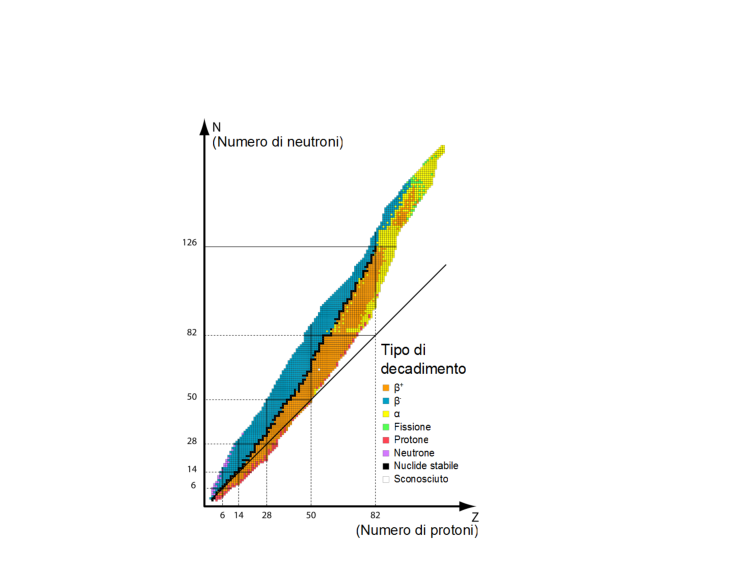
\includegraphics[scale=1]{/nuclei_stabili}
\caption{Il grafico rappresenta per quali combinazioni di neutroni e protoni si hanno atomi stabili.}
\end{figure}
Il decadimento dei nuclei avviene spontaneamente in alcune circostanze

\begin{enumerate}
\item  il nucleo ha troppi neutroni, allora si ha un processo di decadimento beta $\beta^-$
\begin{equation}
^{A}_{Z}X \quad\longrightarrow\quad  ^{A}_{Z+1}X + e^- + \bar\nu_e
\end{equation}
dopo il decadimento si ha un atomo della stessa specie X.
Questo processo è descritto in dettaglio da un decadimento di un neutrone
\begin{equation}
n \quad\longrightarrow\quad p + e^- + \bar\nu_e
\end{equation}
a livello di quark tale processo consiste nella conversione di un quark down in un quark up
\begin{equation}
d \quad\longrightarrow\quad u + e^- + \bar\nu_e
\end{equation}
mediato dal bosone $W$, mediatore della forza debole.

\item il nucleo può avere troppi protoni, si ha allora un processo di decadimento beta $\beta^+$
\begin{equation}
^{A}_{Z}X \quad\longrightarrow\quad ^{A}_{Z-1}Y + e^+ + \nu_e
\end{equation}
dopo il decadimento si ha un atomo di una diversa specie atomica.
Nel dettaglio vediamo che questo processo è descritto dal decadimento di un protone
\begin{equation}
p \quad\longrightarrow\quad n + e^+ + \nu_e
\end{equation}
e a livello di quark 
\begin{equation}
u \quad\longrightarrow\quad d + e^+ + \nu_e
\end{equation}

\item se ci sono troppi nucleoni, quindi siamo nella parte alta del grafico, i nuclei tendono a subire un processo di decadimento alpha $\alpha$, una particella alpha è un nucleo di Elio
\begin{equation}
^{A}_{Z}X \quad\longrightarrow\quad ^{A-4}_{Z-2}Y + \alpha
\end{equation}

\item il nucleo potrebbe avere anche troppa energia, quindi nel caso di un nucleo eccitato $X^{\ast}$, si ha emissione di radiazione elettromagnetica chiamata \emph{radiazione gamma}
\begin{equation}
^{A}_{Z}X^{\ast} \quad\longrightarrow\quad ^{A}_{Z}X + \gamma
\end{equation}

\item nel caso in cui le energie di eccitazione siano molto elevate si può avere decadimento per \emph{fissione} 
\end{enumerate}

Le leggi che descrivono un decadimento impongono la conservazione di 
\begin{itemize}
\item energia
\item quantità di moto
\item carica elettrica
\item numero di nucleoni
\item numero di leptoni
\end{itemize}
la massa invece non si conserva nei processi di decadimento.

\paragraph{esempio:} utilizzando la formula semi-empirica di massa si verifichi se il decadimento $\alpha$ del $^{238}_{92} U$ sia possibile energeticamente.

La massa totale iniziale del sistema deve essere maggiore della massa totale finale, allora il processo è esotermico.
$$ M_i > M_f \quad\Rightarrow\quad esotermico $$
\begin{equation}
^{238}_{92} U \quad\longrightarrow\quad ^{234}_{90}X + ^{4}_{2}He
\end{equation}
dobbiamo calcolare il $Q$ della reazione e ci chiediamo se è maggiore di zero
\begin{equation}
Q = M(A,Z) - M(A-4,Z-2) - M(^{4}_{2}He^{++}) > 0
\end{equation}
la massa dell'atomo iniziale equivale a
\begin{equation}
M(A,Z) = Z M_H + (A-Z)M_n - B(A,Z)
\end{equation}
$B$ rappresenta l'energia di legame
quindi il calore nella reazione è
\begin{equation}
\begin{split}
Q  & = -B(A,Z) + B(A-4,Z-2) + B(^{4}_{2}He^{ ++ }) \\
& = [ -1807.5 + (1784 + 32.85)] MeV = \SI{9.35}{MeV} > 0
\end{split}
\end{equation}
risulta quindi positivo, per cui il decadimento alpha è energeticamente possibile.
La natura tende a minimizzare la massa ed il processo è spontaneo.






